\documentclass[../monografia.tex]{subfiles}

\begin{document}

\section{Revisão da Literatura} 

\section{Indicadores de Qualidade e Conforto} \label{arte-indicadores}

% Separar qualidade e conforto

% Qualidade -> Limites pela legislação e pesquisas
Como qualidade e conforto são termos subjetivos, vamos tratar aqui como "qualidade do ambiente" as condições recomendadas por normas e pesquisas, para os quatro indicadores. Isto é, será considerado um ambiente de boa qualidade o que atender às faixas de operação pré-determinadas, funcionando como um aviso para o ocupante caso as medidas indiquem que os parâmetros do ambiente estão fora do recomendado. 

Já o conforto será atrelado à percepção do usuário quanto ao ambiente. Apesar de o ambiente ser considerado saudável ou de qualidade, existem muitos fatores que afetam a sensação das pessoas, de forma que apenas a definição de uma faixa de operação não implica em bem-estar. 

O conforto e a qualidade em ambientes internos são determinados através de quatro principais indicadores: \textbf{térmico, acústico, luminoso e olfativo/qualidade do ar}\cite{ComfortBox}. 
% citações ??

\subsection{Regulamentações e Normas} %check

A legislação brasileira determina os valores máximos e mínimos dos indicadores de conforto no ambiente para que haja boas condições de trabalho: 

\begin{citacaoLonga} %Normas ministerio
\textbf{NR17 do Ministério do Trabalho} \cite{NR17}

17.5. Condições ambientais de trabalho.

17.5.2. Nos locais de trabalho onde são executadas atividades que exijam solicitação intelectual e atenção constantes, tais como: salas de controle, laboratórios, escritórios, salas de desenvolvimento ou análise de projetos, dentre outros, são recomendadas as seguintes condições de conforto:

a) níveis de ruído de acordo com o estabelecido na NBR 10152, norma brasileira registrada no INMETRO;

b) índice de temperatura efetiva entre 20oC (vinte) e 23oC (vinte e três graus centígrados);

[...]

d) umidade relativa do ar não inferior a 40 (quarenta) por cento.

17.5.2.1. Para as atividades que possuam as características definidas no subitem 17.5.2, mas não apresentam equivalência ou correlação com aquelas relacionadas na NBR 10152, o nível de ruído aceitável para efeito de conforto será de até 65 dB (A)

[...]

17.5.3.3. Os níveis mínimos de iluminamento a serem observados nos locais de trabalho são os valores de iluminâncias estabelecidos na NBR 5413, norma brasileira registrada no INMETRO.
\end{citacaoLonga}

\begin{citacaoLonga} %Normas ABNT

\textbf{NBR 10152} \cite{NBR10152} para Escritórios

Salas de reunião: 30 - 40 dB(A)

Salas de gerência, Salas de projetos e de administração: 35 - 45 dB(A)

Salas de computadores: 45 - 65 dB(A)

Salas de mecanografia: 50 - 60 dB(A)

\textbf{NBR 5413} \cite{NBR5413}

Para escritórios: 500 - 750 - 1000 lux
\end{citacaoLonga}

\subsection{Qualidade do Ar} % Pesquisa CO2 e VOC

% Colocar o que é IAQ, falar sobre?
% Sindrome Predios doentes? -> Intro?
Não há, na legislação brasileira, informações sobre a qualidade do ar. Isto é, concentrações de CO2 e VOC. 

A norma a seguir fala a margem esperada, mas também sem recomendações de operação. 

\begin{citacaoLonga} % ISO IAQ
\textbf{ISO 16017-2:2003}

is applicable to the measurement of airborne vapours of VOCs in a concentration range of approximately 0,002 mg/m3 to 100 mg/m3 individual organic for an exposure time of 8 h
\end{citacaoLonga}

Por conta disso, vamos nos basear em estudos que tentam relacionar as concentrações de CO2 e de VOC com efeitos na saúde e produtividade das pessoas. 

\subsubsection{CO2}
Segundo \cite{AirQuality}, o CO2 apresenta concentrações mais altas em ambientes fechados, esperando-se entre 700 e 2000 ppm, em comparação a cerca de 400ppm em ambientes abertos em áreas urbanas\cite{co2Earth}. 

O CO2, além de ser um gás asfixiante e perigoso em altas concentrações (acima de 40000ppm), também pode afetar a saúde quando em níveis moderados (abaixo de 2000ppm). 
De acordo com o \textit{Winsconsin Department of Health Services}\cite{Winsconsin}, são os efeitos causados na saúde: 
\begin{itemize}
\item 250-400ppm: Normal, concentração ambientes abertos
\item 400-1,000ppm: concentração típica em lugares fechados com pessoas, com boa circulação de ar
\item 1,000-2,000ppm: pode causar cansaço e falta de ar
\item 2,000-5,000 ppm: dores de cabeça, sonolência, e falta de ar mais intensa. Baixa concentração, perda de atenção, aumento da frequência cardíaca, e náusea
\item 40,000 ppm: Pode causar séria insuficiência respiratória, danos permanentes ao cérebro, coma e até a morte
\end{itemize}

\subsubsection{VOC}
Compostos orgânicos voláteis, ou VOC (do inglês,\textit{Volatile organic compounds}, são partículas que ficam suspensas no ar, podendo vir de produtos (sintéticos ou naturais) utilizados no ambiente, como tintas, solventes, produtos de limpeza, perfumes que podem causar odor perceptível pelo ser humano\cite{AirQuality}.

A concentração esperada é entre 0.2 e 0.5 mg/m3, ou entre 62 e 150ppb, e mesmo que nem todos os compostos presentes no ar sejam nocivos à saúde, por precaução é recomendado que estes sigam: \cite{tecam}

\begin{table}[h]
\centering
\begin{tabular}{ |c|c| }
\hline
Nível de TVOC	&   Preocupação \\
\hline
Abaixo de 93 ppb  &  Baixa \\
93 a 150 ppb  &   Pouca \\
150 a 310 ppb &  Moderada \\
310 a 930 ppb &  Alta \\
\hline
\end{tabular}
\caption{Tabela com as concentrações de TVOC e seu impacto }
\label{table}
\end{table}

\subsection{Conforto Visual}

Além da \textbf{intensidade da luz incidente}, cujos níveis são estabelecida na legislação, a \textbf{temperatura da cor} da luz incidente também tem grande relevância. A muitos anos sabe-se que a luz azul emitida, de maior temperatura, causa danos à retina \cite{BlueLight}. \par
% Assim, temperatura é um parâmetro importante para a qualidade do ambiente, muitas vezes deixado de lado, e assim como na saúde, afeta diretamente o conforto e a atenção das pessoas, como visto em \cite{VisualComfort}: 
% \begin{itemize}
% \item Conforto, luz natural: 3000K - 6000K
% \item Concentração: acima de 5300K 
% \end{itemize}


\section{Trabalhos Relacionados a Qualidade de Ambientes Internos} 

O artigo "Development of low-cost indoor air quality monitoring devices:
Recent advancements", de 2020 da Universidade do Porto \cite{IAQ_Compare} traz uma comparação de projetos focados em monitoramento de qualidade do ar. A tabela 2 mostra os estudos que possuem uma maior relevância para o nosso projeto. 

\begin{center}
\begin{longtable}{ |c|c|c| } 
\hline % Cabeçalho
\textbf{Estudo} & \textbf{Parâmetros monitorados} & \textbf{Processador e comunicação} \\ 
\hline %Parkinson 
\multirow{4}{8em}{Parkinson et al.\cite{PARKINSON201915}-\cite{PARKINSON2019241}} & Temperatura, Umidade & ARM-Cortex \\
& CO2, TVOC, CO, Vel. do Ar & On-board e cloud storage \\ 
& Som & LTE \\ 
& Intensidade Luminosa  &  \\ 
\hline % Karami
\multirow{4}{8em}{Karami et al.\cite{KARAMI2018412}} & Temperatura, Umidade & Arduino UNO \\ 
& CO2, VOC & Cloud storage \\ 
& Intensidade Luminosa & Zigbee \\ 
& Ocupação (PIR)  & VOLTTRON Software \\ 
\hline % Carre and Williamson
\multirow{4}{8em}{Carre and Williamson\cite{CARRE20181751}} & Temperatura, Umidade & Arduino Mega 2560 \\ 
& CO2, Vel. do Ar & On-board e cloud storage \\ 
& Intensidade Luminosa & 3G \\ 
& Som, Ocupação (PIR)  &  \\ 
\hline % Tiele
\multirow{3}{8em}{Tiele et al.\cite{Tiele2018}} & Temperatura, Umidade & Feather M0 \\ 
& CO2, TVOC, CO & On-board storage \\ 
& Intensidade Luminosa &  \\ 
\hline % Chanthakit and Rattanapoka
\multirow{3}{8em}{Chanthakit and Rattanapoka\cite{Chanthakit2018}} & Temperatura, Umidade & ESP8266 \\  %!! Colocar na tabela de comunicação
& CO & MQTT Protocol \\ 
&  & \multirow{2}{12em}{Dados não são salvos (projeto futuro)} \\ 
& & \\
\hline % Scarpa et al.
\multirow{4}{8em}{Scarpa et al.\cite{SCARPA2017282}} & Temperatura, Umidade & Arduino \\ 
& CO2 & Onboard e cloud storage \\ 
& Intensidade Luminosa & Wifi (módulo ESP8266) \\ 
& Movimento (IR)  &\\
\hline % Jiang and Huacon
\multirow{3}{8em}{Jiang and Huacon\cite{Jiang2017}} & Temperatura, Umidade & Raspberry Pi 3B \\ 
& CO2 & Cloud storage \\ 
& Som & Thingspeak platform \\ 
\hline %Salamone et al.
\multirow{4}{8em}{Salamone et al.\cite{SALAMONE2017351}-\cite{Salamone2017}} & Temperatura, Umidade & Arduino \\ 
& CO2, Vel. do Ar & On-board e cloud storage \\ 
& Intensidade Luminosa & Wifi shield \\ 
&  & BlueSmiRF (Bluetooth) \\ 
\hline %Ali et el.
\multirow{4}{8em}{Ali et al.\cite{ALI2016114}} & Temperatura, Umidade & Arduino PRO Mini \\
& CO2 & On-board storage \\ 
& Intensidade Luminosa & \multirow{2}{12em}{Sem comunicação wireless (projeto futuro)} \\ 
& Ocupação (PIR) &  \\ 
\hline %Brunelli
\multirow{4}{8em}{Brunelli et al.\cite{Brunelli2014}} & Temperatura, Umidade & Jennic NXP JN5148 %?
SoC \\
& CO2 & Online storage \\ 
& Intensidade Luminosa & IEEE802.15.4/ZigBee \\ 
&  & PRO complaint module \\ 
\hline %Tapashetti
\multirow{3}{8em}{Tapashetti et al.\cite{Tapashetti2016}} & Temperatura, Umidade & (WiFi) Marvell 88 MW302 \\
& CO2, Gas & Cloud storage (AWS) \\ 
& Intensidade Luminosa &  \\ %?
\hline %Marques and Pitarma
\multirow{3}{8em}{Marques and Pitarma\cite{Marques2019}} & CO, CH4, Eth & ESP8266 (Wifi)\\
&  & Cloud storage \\ 
&  & Thingspeak platform \\ 
\hline %Martín-Garín et al.
\multirow{2}{8em}{Martín-Garín et al.\cite{MARTINGARIN2018201}} & Temperatura, Umidade & ESP8266 (Wifi)\\
& CO2 & On-board e Cloud storage \\ 
\hline 
\caption{Tabela comparativa de estudos em dispositivos de monitoramento de ambientes}
\label{table}
\end{longtable}
\end{center}

Podemos ver que as medições mais comuns são de qualidade do ar, e térmica (temperatura e umidade), sendo poucos os estudos onde são realizadas aquisições dos quatro indicadores para ambientes internos. 

Quando há alguma comunicação nos dispositivos, Wi-fi foi a solução mais utilizada, a fim de armazenar os dados coletados em nuvem. Ainda assim, todos os estudos mostravam dispositivos que operam de forma individual, não em rede. 

Não encontramos projetos na literatura que levassem em consideração a sensação de conforto das pessoas, como a coleta de \textit{feedback} proposta. 

\section{Soluções no Mercado} 
% Falar de ser Open Source

A tabela a seguir mostra algumas das principais soluções encontradas no mercado para monitoramento de ambientes fechados: 

\begin{center}
\begin{longtable}{ | m{2.5cm} | m{2.4cm}| m{2.2cm} |m{2cm} |m{2cm} |m{2.8cm} | } 
\hline
\textbf{Projeto} & \textbf{Térmico} & \textbf{Luminoso} & \textbf{Acústico} & \textbf{Ar} & \textbf{Conectividade} \\ 
\hline
Multi comfort \cite{multicomfort} & Sim* & Sim* & Sim* & Sim* & Sim* \\
\hline
MC350\cite{mc350} & Sim* & Sim* & Sim* & & Bluetooth, App \\
\hline
Metriful Sense\cite{metriful} & Temperatura, Umidade, Pressão & Intensidade & Volume, Freq. & VOC & \\
\hline
CoMoS\cite{CoMoS} & Temperatura, Umidade, Veloc Ar & Intensidade & & & Wifi, SW Web \\ 
\hline
HC tech\cite{HCTech} & Temperatura, Umidade & Intensidade & & & Sigfox, SW Web\\ 
\hline
ECOMLITE \cite{ECOMLITE} & Temperatura, Umidade, Pressão & & Volume & $CO_{2}$, CO, VOC, $NO_{2}$ & Wi-fi, Zigbee, Ethernet, SW Web \\ 
\hline
Netatmo\cite{netatmo} & Temperatura, Umidade, & & Volume & CO2 & Wi-fi, App\\ 
\hline
Senlab O\cite{Senlab} & Temperatura, Umidade & Intensidade & & & LoRa \\ \hline
Comfort Click\cite{comfortclick} & Temperatura, Umidade & & Volume & & Wi-fi, App\\ 
\hline
\caption{Tabela comparativa de dispositivos no mercado}
\label{table}
\end{longtable}
\end{center}

\begin{flushright}
(*) Solução não detalhada pela construtora
\end{flushright}

Ao observar as soluções existentes no mercado, é possível ver que a maioria atende a apenas alguns dos indicadores. 

Multi Comfort \cite{multicomfort}, a solução mais completa encontrada, trata-se de uma sistema desenvolvido pela construtora Saint-Gobain de forma integrada à construção do edifício. 
Apesar de atender aos 4 indicadores de qualidade e conforto, essa solução não apresenta detalhes sobre as medições que são feitas, quais os elementos medidos ou a precisão dessas medições, assim como sobre a sua conectividade. 
Além de ser de difícil integração com outros dispositivos do mercado, apresenta grande dificuldade para ser implementado em um ambiente já construído. Nesses contextos, é introduzido o equipamento MC350\cite{mc350} - da mesma empresa -, mas que não atende mais a todos os indicadores. 

Em seguida, temos o Metriful Sense \cite{metriful}, que também atende a todos os indicadores de conforto, que é um produto novo em \textit{crowdfunding}. Diferentemente das demais, esse não é um dispositivo completo, mas uma plataforma de sensores projetada para o monitoramento de ambientes. Necessita de uma interface com outro processador e possivelmente com um módulo \textit{wireless} para que haja conexão com uma plataforma de análise. 

Os demais produtos atendem em média apenas dois dos indicadores de conforto, sendo apenas o conforto térmico presente em todos. 

O conforto luminoso, quando presente, é atendido de forma superficial, sendo medida apenas a intensidade da luz e não a cor da luz, que é um elemento importante na sensação de conforto \cite{VisualComfort}. Já no monitoramento da qualidade do ar, apenas uma das soluções \cite{ECOMLITE} (cuja especificação está disponível) mede ao menos os dois principais elementos indicadores \cite{AirQuality}. 

Vemos, assim como na literatura, que nenhum dos produtos existentes no mercado atende a todos os requisitos levantados para a nossa aplicação. 

Além disso, nenhuma das soluções encontradas envolve diretamente a opinião das pessoas frequentando o ambiente na análise dos seus dados, apenas no controle do ambiente quando esse não atende os requisitos de qualidade ou de conforto. 

Vale destacar, por fim, que na maioria dos casos essas soluções são fechadas, com protocolos que dificultam a integração dos dispositivos com outros que possam complementá-los em seu funcionamento, ou de forma que seja possível uma centralização da análise dos dados coletados. Desenvolvendo um projeto \textit{open-source} e com protocolos padrão de comunicação sem fio, isso deixa de ser um problema. 

\section{Tecnologias Relevantes} 

\subsection{Protocolos de Rede} 

%?? talvez no lugar da frase de iot?
Uma rede de sensores sem fio (WSN, do inglês \textit{Wireless sensor networks}) é composta de vários nós equipados com sensores, processador e um transceptor de rádio. Estes nós podem, assim, coletar informações do ambiente, processar dados e se comunicar com outros dispositivos \cite{wsn-networking}.

Com o crescimento do conceito de Internet das Coisas, novas tecnologias para conexão rápida, segura e fácil de dispositivos são criadas e utilizadas por desenvolvedores em inúmeras aplicações. Segundo a pesquisa \textit{Embedded Markets Study} realizada pela empresa Aspencore\cite{embedded-market-study} e apresentada pelos meios EETimes\cite{eetimes} e Embedded\cite{embedded} em 2019, as interfaces sem fio mais utilizadas por desenvolvedores em  projetos de sistemas embarcados são Wi-Fi, \textit{Bluetooth Low Energy (BLE)} e \textit{Bluetooth Classic}. Essa pesquisa também aponta os protocolos de comunicação sem fio mais utilizados, dentre eles \textit{BLE mesh}, Zigbee, 6LoWPAN e Thread. 

Wi-Fi é o nome dado a uma família de tecnologias designadas para comunicação sem fio baseada no padrão IEEE 802.11\cite{802.11}, amplamente utilizada em redes de área local (em inglês \textit{local area network}, LAN) para prover acesso à internet como uma alternativa à tecnologia cabeada Ethernet. Essa tecnologia opera nas faixas de 2,4GHz e 5GHz, sendo que a primeira permite uma taxa de transmissão de até 600 Mbits/s e a segunda até 1 Gbit/s em casos mais extremos\cite{Wi-Fi-datarate}. A topologia comum de uma rede Wi-Fi é dada por um  dispositivo que atua como ponto de acesso que disponibiliza o sinal sem fio para que dispositivos ao seu redor possam se conectar à rede, em uma topologia de rede em estrela. Deste modo, os dispositvos têm que estar a uma distância de poucos metros do ponto de acesso para que a comunicação não seja afetada, sendo essa distância cerca de 76m a 122m em ambientes internos\cite{wifi-range}, dependendo da antena utilizada.

Outra norma comumente utilizada em redes sem fio é a IEEE 802.15.4, que define especificações de camada física e de enlace da pilha de protocolos OSI para redes de comunicação sem fio que operam com baixa taxa de transmissão de dados (em inglês, \textit{Lower Rate Wireless Personal Area Network,}, ou LR-WPAN), que também utiliza a banda de frequência de 2,4GHz\cite{802.15.4}. Os nós participantes da rede podem ser do tipo "função completa" (FFD, do inglês \textit{full-function device}), agindo como coordenador da rede, podendo retransmitir mensagens para outros nós, ou do tipo "função reduzida" (RFD, do inglês \textit{reduced-function device}, destinados a serem dispositivos simples e com poucos requisitos de comunicação, podendo apenas se comunicar com FFDs, possibilitando aplicações com menor custo energético. 

Por último, dentre as tecnlogias citadas anteriormente, o Bluetooth surgiu com objetivo de substituir a conexão por fios entre dispositivos móveis comuns como celulares e fones de ouvido, porém já evoluiu muito e pode ser encontrada em diversas aplicações. O IEEE padronizou a tecnologia como IEEE 802.15.1, mas atualmente mantinda por outra organização, a \textit{Bluetooth Special Interest Group} (Bluetooth SIG), composta por mais de 35 mil empresas parceiras, que gerencia o desenvolvimento e define os padrões da tecnologia. Em 2009, a Bluetooth SIG definiu uma nova versão de baixo consumo energético, chamada de \textit{Bluetooth Low Energy} (BLE), visando aplicações em que não é necessária comunicação contínua como, por exemplo, sensores que coletam dados em intervalos de tempo espaçados. O BLE vem se tornando uma das principais tecnologias para aplicações IoT, principalmente por estar presente na maioria dos dispositivos mais comuns utilizados no dia-a-dia das pessoas, como computadores, \textit{smartphones} e \textit{tablets}, o que facilita a comunicação do usuário com outros dispositivos específicos. As aplicações BLE operam de 2,4 a 2,485GHz com taxas de transmissão entre 0,27 e 1,37 Mbps\cite{ble-datarate}. 

\subsection{Protocolos de Aplicação} \label{protocolos-aplicacao}

O protocolo BLE possui uma especificação que engloba desde a camada física até a de aplicação, como mostrado na figura \ref{fig:ble-stack}, diferentemente dos outros dois protocolos apresentados. 

\begin{figure}[h]
\centering
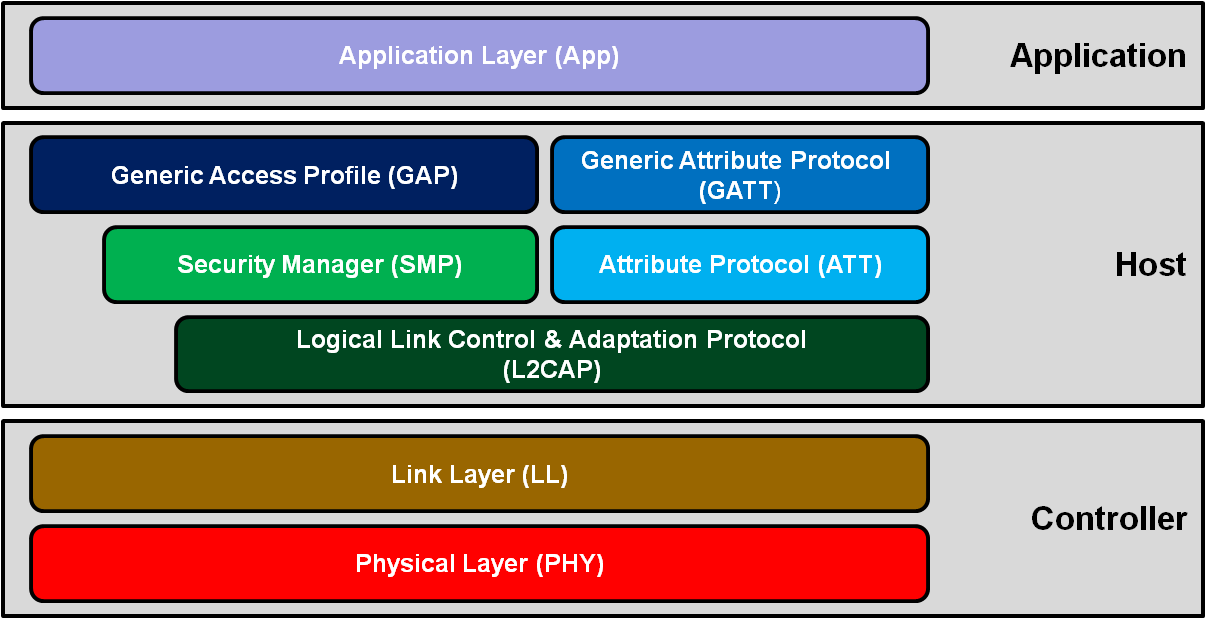
\includegraphics[scale=0.6]{ble-protocol-stack.png}
\caption{Arquitetura em camadas do protocolo BLE. Retirado de \cite{ble-protocol-stack}}
\label{fig:ble-stack}
\end{figure}

Para o caso do WiFi no contexto de IoT, em que dispositivos simples e com pouca capacidade de processamento, como sensores, precisam estar conectados à servidores via Internet, há a necessidade do uso  de protocolos de aplicação também mais simples. O protocolo HTTP é um dos principais protocolos de aplicação utilizados na Web, porém possui algumas características que o tornam não muito adequado para aplicações nesse contexto, como a necessidade de longos cabeçalhos e regras antes do corpo da mensagem, que podem ocasionar \textit{overheads} quando tratamos que dispositivos com pouca capacidade de processamento, a necessidade do cliente esperar por uma resposta do servidor e a comunicação ser unidirecional, sempre iniciada pelo cliente para o servidor.

Um protocolo comumente utilizado em aplicações IoT é o \textit{Message Queuing Telemetry Transport} (MQTT) \cite{mqtt-specification}, implementado sobre a pilha TCP/IP, criado pela IBM em 1999, que utiliza o modelo \textit{Publisher/Subscriber}, onde dispositivos MQTT publicam mensagens em tópicos em um dispositivo centralizado, chamado \textit{Broker}, e se inscrevem em outros tópicos para receberem mensagens. O papel do \textit{Broker} é receber as mensagens publicadas nos diferentes tópicos e redirecioná-las para os dispositivos que estão inscritos nesses tópicos. Desse modo, o protocolo MQTT apresenta grande escalabilidade, facilitando a implementação de redes com muitos dispositivos. É um protocolo orientado à conexão, já que a comunicaçao entre Cliente e \textit{Broker} utiliza TCP na camada de transporte, podendo também ser utilizado TLS/SSL para segurança. 

Visando utilizar a arquitetura de APIs REST presentes na Web em redes de dispostivos com baixa capacidade de processamento, facilitando a interoperabilidade com HTTP, o grupo de trabalho CoRE (\textit{Constrained RESTful Environments}) do IETF definiu o protocolo CoAP (\textit{Constrained Application Protocol}) no RFC7252 \cite{coap-specification}. O CoAP faz uso do UDP, com cabeçalho fixo de 4 bytes, fazendo com que os datagramas sejam relativamente pequenos, dependendo apenas do tamanho da mensagem a ser transmitida, e tornando a comunicação mais leve, já que o UDP, diferente to TCP, não é voltado à conexão, ou seja, nenhum tipo de \textit{handshake} precisa ser estabelecido entre os dispositivos. Isso possui um lado negativo, que é uma confiabilidade menor na entrega dos dados pela camada de transporte, sendo que o mecanismo de confiabilidade de dados precisa ser implementado na própria camada de aplicação. Assim como no HTTP, são definidas requisições GET, POST, PUT e DELETE para interação entre os dispositivos através de URIs, porém quem atua como servidor é o próprio dispositivo IoT, recebendo as requisições de um agente externo e respondendo adequadamente com os dados requisitados, o que facilita o gerenciamento de uma rede com vários dispositivos. 

O artigo \cite{mqtt-coap-comparison} faz a uma comparação desses protocolos, adicionando ainda um quarto, o AMQP, resumida na tabela \ref{table:mqtt-coap-comparison}.

\begin{table}[h]
\centering
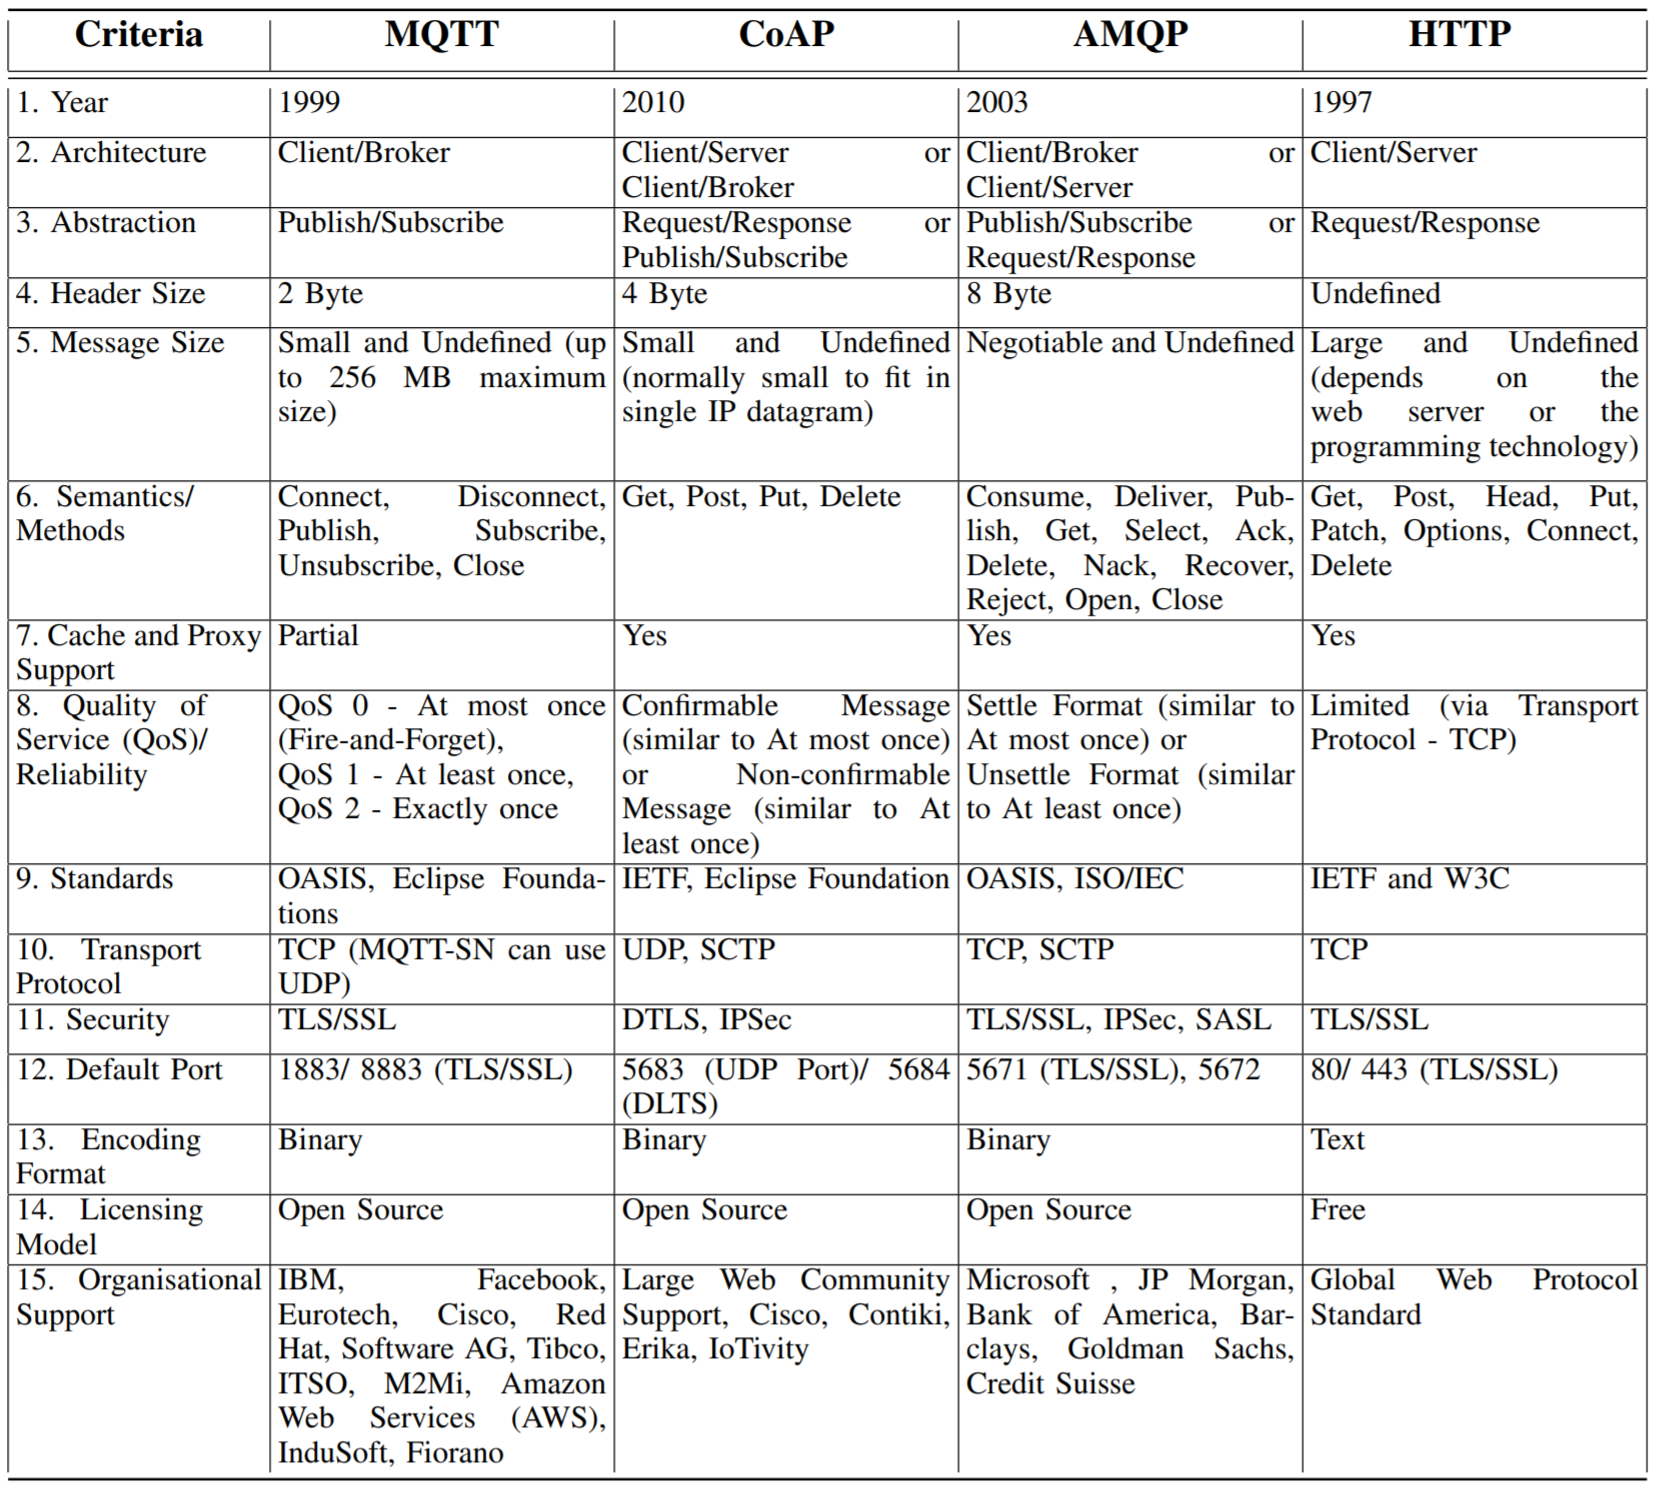
\includegraphics[scale=0.4]{comparacao-mqtt-coap-http.png}
\caption{Análise Comparativa de Protocolos de Comunicação para Sistemas IoT: MQTT, CoAP, AMQP e HTTP. Retirado de \cite{mqtt-coap-comparison}}
\label{table:mqtt-coap-comparison}
\end{table}


** OBS: Mostrar tecnologias de aplicação baseadas no 802.15.4, como zigbee e thread **
 
\subsection{Topologias de Rede} \label{topologias-rede}

Os protocolos de rede citados possuem, em geral, topologias de rede baseadas em estrela, com vários dispositivos periféricos conectados a um central, ou em árvore, que pode ser vista como várias redes em estrela interconectadas. No segundo caso, apenas os dispositivos centrais de cada rede em estrela poderia se comunicar com as outras, atuando como um dispositivo de borda. Desse modo, a conexão entre dispositivos periféricos e central da rede se dá de forma ponto-a-ponto, o que gera uma dependência forte do central e, caso ele apresente algum problema, pode afetar o funcionamento da rede inteira.

\begin{figure}[h!]
\centering
\begin{minipage}{.5\textwidth}
	\centering	
	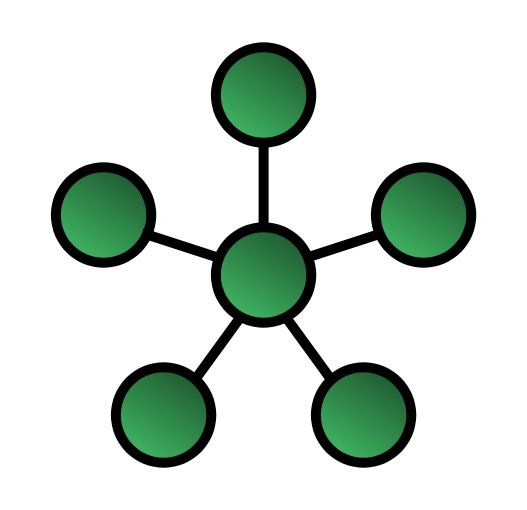
\includegraphics[width=.4\linewidth]{star-network}
	\caption{Topologia de rede em estrela}
	\label{fig:Rede em estrela}
\end{minipage}%
\begin{minipage}{.5\textwidth}
	\centering
	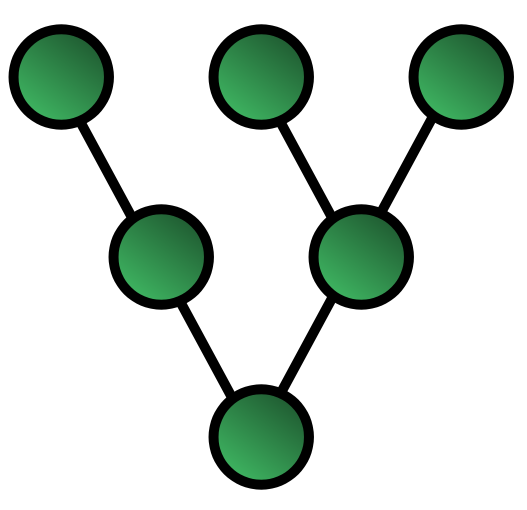
\includegraphics[width=.4\linewidth]{tree-network}
	\caption{Topologia de rede em árvore}
	\label{fig:Rede em árvore}
\end{minipage}

\end{figure}


O crescimento e evolução das aplicações IoT requer topologias mais novas e complexas, com a capacidade de se ajustarem dinamicamente caso ocorra alguma mudança na rede. Com isso em mente, soluções de redes em malha começam a surgir nos protocolos anteriormente citados. Nessa topologia, os nós ficam interligados de forma não-hierárquica, permitindo a comunicação \textit{many-to-many} entre os dispositivos da rede, possibilitando que dados de um ponto qualquer seja enviado a outro ponto qualquer da rede. 


\begin{figure}[h!]
\centering
	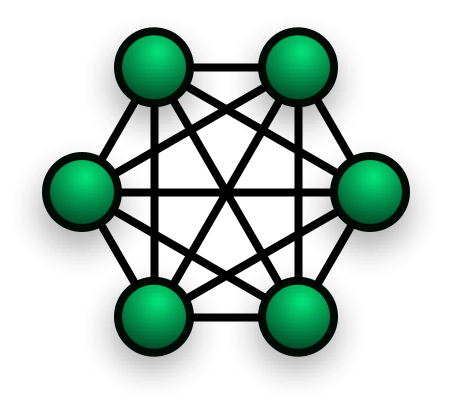
\includegraphics[scale=.2]{mesh-network}
	\caption{Topologia de rede em malha}
	\label{fig:Rede em malha}
\end{figure}

Dada essa necessidade, as epecificações dos protocos de comunicação começaram a adicionar soluções de rede em malha, como BLE Mesh, 802.11s (Wi-Fi mesh) e Thread, que é construída em cima da especificação 6LoWPAN. O protocolo Zigbee já possui suporte a redes em malha desde sua primeira concepção. Essas definições são feitas a nível da camada de rede, se utilizando das especificações das respectivas tecnologias para implementar novas maneiras de roteamento de dados entre os dispositivos.

O artigo \textit{Wireless Mesh Networking: An IoT-Oriented Perspective Survey on Relevant Technologies}, publicado pela \textit{Future Internet}\cite{mesh-net-comparison} faz uma análise comparativa entre diferentes tipos de protocolos de comunicação atuando na topologia de rede em malha: família IEEE 802.15.4 (Zigbee e Thread), IEEE 802.11 (em especial a IEEE 802.11s que define redes em malha), LoRa Mesh e IEEE 802.15.1 (BLE Mesh).

\begin{figure}[h!]
\centering
	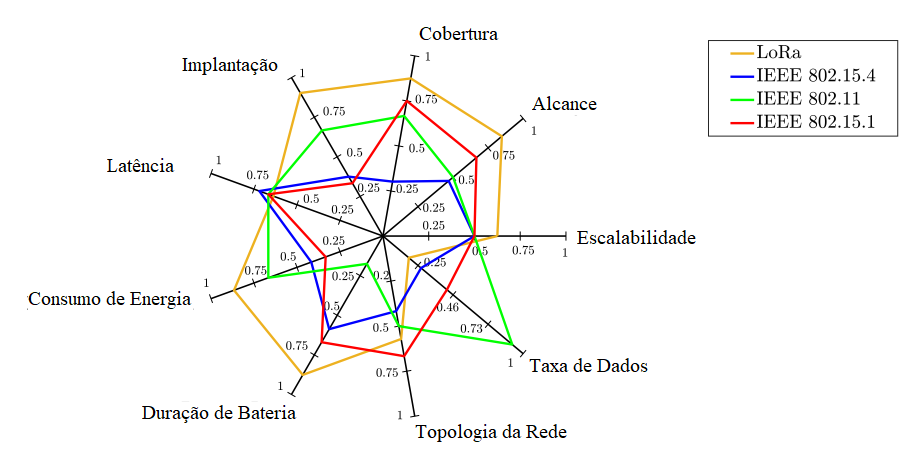
\includegraphics[width=\textwidth]{mesh-net-comparison}
	\caption{
		Comparação de performance entre 4 tecnologias de rede sem fio, em topologia de malha, de acordo com 9 parâmetros. Retirado de \cite{mesh-net-comparison} (traduzido).
	}
	\label{fig:Comparação redes mesh}
\end{figure}

O gráfico mostrado na figura \ref{fig:Comparação redes mesh}  pode ser utilizado para resumir de maneira completa a pesquisa realizada em \cite{mesh-net-comparison}. O protocolo LoRa foge do escopo deste projeto, pois é destinado para comunicações entre distâncias quilométricas e possui taxa de transmissão de dados muito baixa, por isso será desconsiderado como alternativa para a aplicação deste projeto. É possível observar os seguintes pontos:

\begin{itemize}
	\item A tecnologia Wi-Fi é claramente a que possui maior taxa de transmissão de dados, com área de cobertura e alcance razoáveis, mas com a desvantagem de possuir um consumo de energia elevado.
	\item Redes BLE Mesh são as mais eficientes em termos de consumo de energia, mostrado também no artigo \cite{zigbee-ble-power}, possuem grande área de cobertura, já que uma rede pode possuir até 32 mil nós\cite{BLE-mesh}, e possuem uma taxa de trasmissão de dados alta, comparada com as soluções baseadas na IEEE 802.15.4.
	\item Todas as soluções apresentadas possuem alta escalabilidade e níveis de latência comparáveis.
\end{itemize}


\subsection{Redes Bluetooth Mesh}

Como citado anteriormente, \textit{Bluetooth Mesh} é um padrão de rede em malha baseado no protocolo \textit{Bluetooth Low Energy} (BLE) com a finalidade de permitir a comunicação do tipo \textit{many-to-many} entre os dispositivos de uma mesma rede. Essa tecnologia se baseia nos seguintes princípios:

\begin{itemize}
	\item \textit{milti-hop}: mensagens enviadas são reencaminhadas por vários outros dispositivos até que atingam seu destino, permitindo que os dispositivos de orgigem e destino não estejam diretamente interconectados, o que possibilita criação de redes extensas.
	\item \textit{multi-path}: cópias de uma mensagem são enviadas por diversos caminhos diferentes até chegar ao destino, sendo a primeira a chegar processada e as outras cópias descartadas, provendo redundância de dados no nível de rede.
	\item \textit{milticast}: dispositivos usualmente enviam uma mesma mensagen para vários destinos diferentes.
\end{itemize}

O padrão foi idealizado visando possibilitar e encorajar interoperabilidade de dispositivos totalmente diferentes, desenvolvidos por diferentes fabricantes, como, tomando como exemplo um prédio inteligente, sensores que medem o estado atual do ambiente e enviam mensagens para controlar equipamentos de ar condicionado, cortinas e luzes inteligentes, bastando seguir as normas especificadas pela Bluetooth SIG de comunicação. Uma dessas padronizações é a definição de mensagens que serão compartilhadas entre os nós da rede. Cada nó possui estados que definem sua condição condição atual --- ligada ou desligada, no caso de uma lâmpada --- e, para que outro nó possa interagir com este, ele pode enviar mensagens que vão altererar ou ler o valor atual de tal estado. São elas:

\begin{itemize}
	\item \textbf{SET}: mensagens desse tipo servem para alterar o valor do estado
	\item \textbf{GET}: enviada por um nó para ler o valor de um estado de outro nó
	\item \textbf{STATUS}: utilizada por um nó para notificar outros nós o valor do seu estado atual
\end{itemize}

Cada elemento de uma rede possui um endereço específico que o identifica, utilizado por outros nós para o envio de mensagens. Porém, a especificação também define o modelo de comunicação \textit{Publish/Subscribe}, onde são definidos grupos com endereços fixos em que os nós podem publicar mensagens ou se inscrever para receber todas as mensagens publicadas nesse endereço. Isso faz com que, em redes grandes, não seja necessário saber o endereço de cada nó especificiamente pra o envio de mensagens, apenas os endereços dos grupos que cada nó deve publicar suas mensagens ou se increver, permitindo trocar dispositivos da rede em caso de problemas sem que a funcionalidade da rede seja afetada, bastando apenas manter os endereços dos grupos pré-definidos.

\begin{figure}[h!]
	\centering
	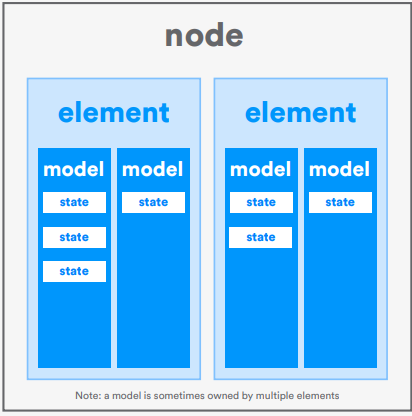
\includegraphics[scale=0.85]{ble-mesh-node-composition.png}
	\caption{Composição lógica de um nó BLE Mesh. Retirado de \cite{ble-mesh-models}}
	\label{fig:ble-mesh-node-composition}
\end{figure}

A estrutura lógica de um nó da rede está representada na figura \ref{fig:ble-mesh-node-composition}. Podemos dizer que um nó na rede equivale a um conjunto de um ou mais \textbf{elementos} (ou \textit{elements}, em inglês), que é a estrutura logica endereçável na rede, sendo que cada elemento em si é constituido por um ou mais \textbf{modelos} (ou \textit{models}). Dessa forma, um nó (dispositivo físico) pode conter vários elementos que definem diferentes funcionabilidades lógicas para esse dispositivo. Modelos são estruturas padronizadas que realizam um tipo especifico de tarefa, constituídos por estados que o definem e mensagens pré-estabelecidas utilizadas para a interação com outros Modelos.

Seguindo a especificação, os Modelos podem ser do tipo \textbf{Cliente}, que não possuem estados e servem apenas para interagir com os Modelos do tipo \textbf{Servidor}, os quais possuem estados. O exemplo mais comum dessa definição é o caso de um interruptor interagindo com uma lâmpada: o interruptor implementaria o \textit{Generic OnOff \textbf{Client}} e a lâmpada o \textit{Generic OnOff \textbf{Server}}, dado que quem possui o estado de ligada ou desligada é a lâmpada (servidor), alterado ou lido pelo interruptor (cliente).

Para que um dispositivo faça parte de uma rede e possa se comunicar dentro desta, ele necessita de uma chave específica, utilizada para criptografar todas as mensagens enviadas dentro de tal rede, chamada de Chave de Rede (\textit{Network Key}, em inglês, ou NetKey). Esta chave é única e serve para definir uma rede específica. Todos os dispositivos que possuirem essa chave conseguem se comunicar entre si. Um mesmo dispostivo pode fazer parte de mais de uma rede, possuindo assim mais de uma NetKey. Além disso, os Modelos precisam de uma outra chave para interagir com os outros, chamada de Chave de Aplicação (\text{Application Key}, em inglês, ou AppKey), de forma que apenas os Modelos que possuírem a mesma AppKey conseguem se comunicar. Esse conceito torna possível a criação de suberedes dentro de uma mesma rede BLE Mesh para diferentes aplicações, como separar dispositivos em cômodos de uma casa, diferentes salas em um prédio etc.

O processo de definição de quais redes o dispositivo fará parte (atribuindo-o as chaves necessárias) e quais os endereços que ele deve se inscrever e publicar mensagens é chamado de \textbf{Provisionamento}, realizado por um dispositivo especial com o papel de \textbf{provisionador}, sendo este o definidor incial de uma rede e suas chaves. Normalmente, esse dispositivo é um \textit{smartphone} que permite um controle mais interativo pelo usuário, mas pode ser também qualquer outro dispositivo que esteja equipado com essa função. Como mencionado, o processo de provisionamento consiste em atribuir a NetKey que define a rede ao dispositivo, assim como quais Modelos possuirão determinadas AppKeys.

O Bluetooth SIG define 52 Modelos padrões, listados e especificados em \cite{BLE-mesh}, divididos em quatro grandes grupos: modelos genéricos, modelos para sensores, modelos específicos para aplicações de iluminação e modelos relacionados a controle de tempo. Também podemos notar que todo Modelo Servidor possui um Modelo Cliente correspondente e vice-versa. Além desses modelos padrões, desenvolvedores podem projetar seus próprios modelos customizados, chamados de Modelos de Fornecedores (\textit{Vendor Models}, em inglês), sendo necessário definir tanto o formato de dados que eles possuirão (Estados) e as mensagens que devem ser utilizadas para interagir com esse modelo.

Exitem bilhões de dispositivos que implementam o protocolo Bluetooth sendo produzidos todo ano \cite{ble-market-update}, porém muitos deles não são capazes de fazer parte de uma rede BLE Mesh nativamente, seja por não possuírem as camadas necessárias por escolha dos desenvolvedores, ou por simplesmente terem sido produzidos antes da especificação ser concluída. Para aproveitar essa grande quantidade de dispostivos presentes no mercado e tornar possível a interação deles com redes BLE Mesh, existe um tipo especial de dispositivo que pode estar presente na rede, chamado \textit{\textbf{Proxy}}, capaz de se comunicar através da especificação do BLE Mesh e pelos perfis GATT \cite{BLE-GATT} ao mesmo tempo, "traduzindo" mensagens presentes na rede mesh para que esses dispositivos BLE possam também fazer parte da rede. Essa implementação é a que torna possível que um \textit{smartphone} atue como um dispositivo provisionador, como citado anteriormente, que faça o papel de Cliente para acender luzes inteligentes em uma casa ou faça requisições para obter dados dispositivos com sensores, facilitando a interação de um usuário comum com diversas implementações de redes. O fato de que quase toda pessoa que possui um \textit{smartphone} é capaz de interagir com qualquer rede BLE Mesh de forma nativa é um dos fatores que tornam essa tecnologia muito promissora para aplicações voltadas diretamente aos usuários, como dispositivos conectados em \textit{smart homes} e \textit{smart buildings}.



\end{document}